% !TeX root = ../Book1.tex
\begin{tikzpicture}[>=stealth,font=\small,x=6cm,y=3cm]
	\draw[gray,dashed] (-.16,0)--(1.17,0) node[right] {\(y=0\)};
	\draw[gray!55,dotted] (0,0)--(0,.3333);
	\draw[gray!55,dotted] (.5,0)--(.5,-.3333);
	\draw[gray!55,dotted] (1,0)--(1,.3333);
	\draw[->,thick,blue!70!black,shorten >=3pt,shorten <=3pt] (0,.3333)--(.5,-.3333) node[midway,below left] {\(s\)};
	\draw[->,thick,blue!70!black,shorten >=3pt,shorten <=3pt] (.5,-.3333)--(1,.3333) node[midway,below right] {\(s\)};
	\draw[->,thick,red!70!black,shorten >=3pt,shorten <=3pt] (0,.3333) to[bend left=30] node[above] {\(s^2=\tau_{(1,0)}\)} (1,.3333);
	\foreach \p in {(0,.3333),(.5,-.3333),(1,.3333)} {
		\fill[blue!70!black] \p circle (1.8pt);
	}
	\node[left] at (0,.3333) {\(p\)};
	\node[below] at (.5,-.3333) {\(sp\)};
	\node[right] at (1,.3333) {\(s^2p\)};
	\node[below] at (0,0) {\(0\)};
	\node[above] at (.5,0) {\(\tfrac12\)};
	\node[below] at (1,0) {\(1\)};
\end{tikzpicture}
